% software flow chart
% -------------------

\documentclass[border=0mm,tikz]{standalone}
\usepackage[utf8]{inputenc}
\usetikzlibrary{mindmap}
\usetikzlibrary{positioning}
\usetikzlibrary{fit}
\usetikzlibrary{scopes}

\begin{document}
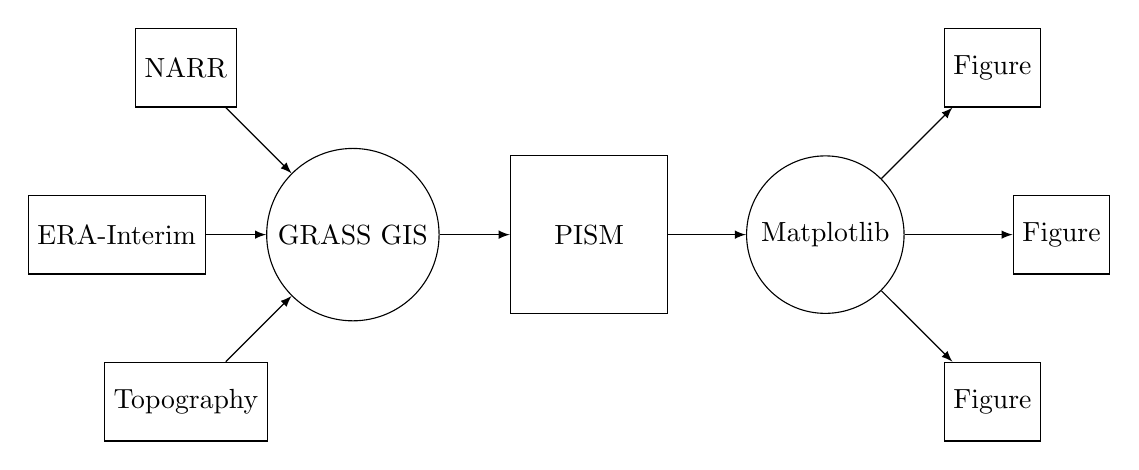
\begin{tikzpicture}[node distance=3cm]
  \tikzstyle{data}=[rectangle, minimum size=1cm, draw]
  \tikzstyle{soft}=[circle, minimum size=2cm, draw]
  \tikzstyle{pism}=[rectangle, minimum size=2cm, draw]
  \node [pism] at (0,0) (pism) {PISM};
  \node [soft] [      left of = pism] (grass) {GRASS GIS};
  \node [data] [above left of = grass] (clim1){NARR};
  \node [data] [      left of = grass] (clim2){ERA-Interim};
  \node [data] [below left of = grass] (clim3){Topography};
  \node [soft] [      right of = pism] (plot) {Matplotlib};
  \node [data] [above right of = plot] (fig1) {Figure};
  \node [data] [      right of = plot] (fig2) {Figure};
  \node [data] [below right of = plot] (fig3) {Figure};
  \draw[-latex] (clim1) -- (grass);
  \draw[-latex] (clim2) -- (grass);
  \draw[-latex] (clim3) -- (grass);
  \draw[-latex] (grass) -- (pism);
  \draw[-latex] (pism) -- (plot);
  \draw[-latex] (plot) -- (fig1);
  \draw[-latex] (plot) -- (fig2);
  \draw[-latex] (plot) -- (fig3);
\end{tikzpicture}

\end{document}
